\scanpage{17}
Sur les groupes de Galois attachés aux groupes $p$-divisibles\hfill 131

spéciale aux groupes de dimension 1). On en déduit que \textit{$I$ est un sous-groupe ouvert de $G$}; je ne connais pas de démonstration directe de ce fait.

3) Le groupe $I$ possède deux filtrations naturelles $v$ et $w$, définies de la manière suivante:
\[
\begin{aligned}
v(g)\geq n&\Leftrightarrow(g-1)(T)\subset p^nT,\\
w(g)\geq n&\Leftrightarrow g\in I^n
\end{aligned}
\]
($I^n$ désigne le $n$-ème groupe de ramification de $I$, dans la notation supérieure, cf. [6], chap. IV, \S\ 3).

Quelle relation y a-t-il entre $v$ et $w$? Si $e_K$ désigne l'indice de ramification absolu de $K$, est-il vrai que l'on a
\[
w=e_K\cdot v+O(1)?
\]
Une question analogue se pose pour tous les groupes de Lie $p$-adiques qui sont des groupes de Galois.
\margin{\figure{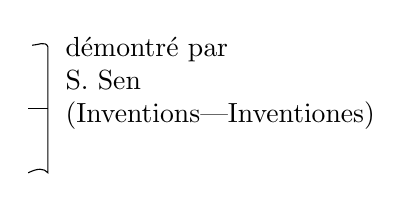
\begin{tikzpicture}[x=1cm,y=1cm]
\draw (0,0) .. controls (.12,.06) and (.2,.06) .. (.25,0) -- (.25,1.6) .. controls (.22,1.68) and (.12,1.62) .. (.05,1.62);
\draw (0,.82)--(.25,.82);
\node[anchor=north west,align=left] at (.35,1.85) {démontré par\\S. Sen\\(\unsure{Inventions|Inventiones})};
\end{tikzpicture}}}

\begin{center}\textbf{Bibliographie}\end{center}

[1] \textsc{Chevalley}, C.: Théorie des groupes de LIE, II et III. Publ. Inst. Math. Univ. Nancago, Paris: Hermann 1951 et 1955.

[2] \textsc{Lubin}, J.: One-parameter formal LIE groups over $p$-adic integer rings. Ann. of Maths. \textbf{80}, 464--484 (1964).

[3] \textsc{Lubin}, J.: Finite subgroups and isogenies of one-parameter formal LIE groups. Ann. of Maths. \textbf{85}, 296--302 (1961).

[4] \textsc{Mumford}, D.: Geometric invariant theory. Ergeb. der Math., Neue Folge, Bd. 34. Berlin, Heidelberg, New York, Springer 1965.

[5] \textsc{Mumford}, D.: Families of abelian varieties. Algebraic groups and discontinuous subgroups. Proc. Symp. Pure Maths. \textbf{9}, A.M.S. (1966).

[6] \textsc{Serre}, J-P.: Corps Locaux. Publ. Inst. Math. Univ. Nancago, VIII, Paris: Hermann 1962.

[7] \textsc{Serre}, J-P.: LIE algebras and LIE groups. New York: Benjamin 1965.

[8] \textsc{Serre}, J-P.: Résumé des cours 1965--66. Annuaire du Collège de France, 49--58, (1966--67).

[9] \textsc{Tate}, J.: $p$-divisible groups, ce volume p. 158--183.
\margin{16}
